\section{О честных выборах}

Отвлечёмся немного от теории и обратимся к теме, которая на первый взгляд к серьёзной математике почти не имеет отношения: к политическим выборам. Сделаем мы это с одной стороны ради чистого интереса и веселья, а с другой стороны для того, чтобы на простом интуитивном примере ввести понятие \term{ультрафильтров}, которые впослеедствии постужит нам добрую службу. Материал этого параграфа строго не обязателен для изучения (тем более упражнения), за исключения заключительной части, вводящей определения фильтров и ультрафильтов.

Предположим, что у нас имеется кандидат в президенты, которого готовы отдать голоса 26\% избирателей. Вслед за ним идёт кандидат с 12\%, за ним с 11\% и дальше идёт большое количетво кандидатов, за которые готовы голосовать менее 10\% населения. Предположим теперь, что самый популярный кандидат~--- фашист, людоед и сволочь, и в общем-то кроме 26\% его сторонников никто больше за него голосовать не стал бы и вообще в страшном сне видит его победу. Одна проблема: его противники разбиты на разные идеологические лагери и не имеют единого кандидата. Может быть большинство голосует даже не за своего кандидата, а "лишь бы против людоеда". Вот только против они голосуют неорганизованно. По результатам выборов простым большинством людоед побеждает, хотя это совершенно не отражает волю большинства.

Чтобы таких исторических трагедий не происходило, была придумана двухступенчатая система голосования. В первом этапе голосования определяются два фаворита, а во вотором туре голосовать можно уже только за одного из лидеров. Назовём условно кандидата с 12\% голосов <<либералом>>. Не смотря на то, что в первом туре он значительно уступает людоеду, они оба проходят во второй тур, и уже во втором туре все противники канибаллизма голосуют за либерала. Не потому что он очень им нравится, а потому что они не хотят допустить фашиста во власть. Итог: либерал побеждает с 74\% голосов против всё тех же 26\% у фашиста.

Вроде бы нас двухступенчатая система спасла от трагедии. Но так ли хороша она на самом деле? Фашист ведь не дурак, и при наличии поддержки его значительной долей избирателей, он может ввести на выборы своего искусственного оппонента, а в действительности единомышленника. Если он так поступит, то, скажем, половина избираталей уйдёт к <<аппоненту>> и оба получат примерно по 13\% голосов. Это всё равно больше, чем у либерала, и в итоге во второй тур проходят два практически идентичных людоеда, один из которых становится президентом, а второй премьер-министром.

Такое большое преимущество конечно радко случается, хотя бывает. Предположим, что за фашиста отдают голоса всего 14\% населения. В этом случае ему победить будет уже сложнее, но он всё равно имеет возможность манипулировать выборами. Фашист может создать искуственного конкурента своему наиболее опасному аппоненту, введя на выборы ещё одного либерала. Пусть этот второй либерал не будет популярен, но даже если он отъест хотя бы 2\% от первого либерала, во второй тур либералы уже не пройдут. А кандидат, следующий за либералом с 11\% голосами, вероятно, очень слаб. Например, он сталинист или ЛГБТ-активист, а в России многие предпочтут голосовать скорее за фашиста, нежели за гомосексуалиста (все же нормальные пацаны). Опять же фашист побеждает.

Помимо того, что кандидаты в президенты могут манипулировать выборами, вводя своих фиктивных кандидатов, сами избиратели так же действуют часто тактически. При двуступенчатой системе голосования у действительно симпатичного кандидата редко есть хоть какие-либо шансы на успех и поэтому голосовать за него нет смысла. Куда полезнее определиться с тем, чью победу допускать не хотелось бы вообще никак и бороться против него. В этом случае избирателю разумно определить список хоть как-то приемлемых кандидатов, оценить того, у которого наивысшие шансы на проход во второй тур, и голосовать за него. Многие исследования подтверждают, что в большинстве случае именно так и происходит: люди голосуют не за своего кандидата, а за самого серьезного оппонента тому, кто им неприятен.

Наиболее подвержденны такитческим голосованиям выбора в парламен, который как правило формируется пропорционально: какая доля населения отдала свои голоса за партию, такую долю партия и получит в парламенте. При этом доля может быть не произвольной, а существует некий <<проходной барьер>>. В России, например, этот барьер составляет 5\%, и если партия не получает 5\% голосов, то она вообще не получает представительства в Думе. Необходимость в каком-либо барьере существует чисто техническая: если в парламенте имеется всего 100 мест, а партия набрала 5 голосов из двух миллионов, то очевидно, что места ей не хватит. Другое дело, что правительство часто завышает барьер куда выше, нежели того требуют технические соображения. Цель, которая при этом преследуется, официально состоит в том, чтобы избежать дробления парламента на маленькие фракции и тем самым позволить парламенту более эффективно работать, а так же в том, чтобы не допустить в парламент радикалов, маргиналов и экстремистов.

На практике часто получается так, что проходной барьер оказывается средством манипулирования выборами. На выборах в ГосДуму в 1995 году 45\% голосов набрали те партии, которые не смогли предолеть пятипроцентного барера. Таким образом мнение половины населения при распределении мест в Думе было вообще никак не учтено и парламентские места по сути были отданы людям, против которых голосовала половина населения. На выборах 2011 года проходной барьер был повышен до 7\%, что по сути перекрывало путь в правительство любым оппозиционным партиям.

Процентный барьер могут использовать не только политические партии в своих целях, он так же предполагает широкие возможности по тактическому голосованию для избирателей. Предположим, что на 100 мест парламента претендует четыре партии~--- две партии имеют по 44\% голосов, одна оппозиционная партия 8\% голосов и одна оппозиционная 4\%. При проходном барьере в 5\% последняя партия не проходит в парламент. После голосования без учёта проигравшей партии, две крупных партии получат по 46 мест каждая, и оппозиционная партия, прошедшая барьер получит 8 мест.

Предположим теперь, что часть оппозиционеров (скажем, 2\%) решила отдать свои голоса менее популярной партии. В этом случае обе партии получают по 6\% и обе проходят в парламент. На каждую партию получается меньше мест (6 вместо восьми), однако в сумме оппозиция представлена уже 12-ю парламентариями, а не 8-ю. Крупным партиям так же приходится немного стесниться: вместо 92 мест на двоих они теперь имеют только 88 мест.

Понятно, что когда политики пытаются манипулировать выборами~--- это плохо. Но на самом деле так же плохо и когда избиратели манипулируют выборами, так в этом случае выборы превращаются из процесса определения мнения населения в интеллектуальную стратегическую игру где побеждает не тот, кто дейстивительно предпочтителен обществом, а тот, кто переиграл оппонента. Это явно не соответствует заявленной цели демократических выборов.

Проблема тут кроется не в избирателях или политиках, которые манипулируют выборами, а в самих правилах игры. Как мы видели, двухступенчатые выборы могут защитить нас от ситуации, при которой побеждает наименее желательный кандидат. Можно придумать и другие системы выборов, которые ещё более надёжды.

Простейшая система голосований~--- <<\term{одобрительные выборы}>>, когда избиратель указывает в биллютене не лучшего по его мнению кандидата, а ставит галку напротив всех тех кандидатов, которые в принципе ему приемлемы. Кандидат, который примлем по мнению большинства избирателей, побеждает. При такой системе выборов введение любых новых кандидатов на выборы никак не может повлиять на выбор победителя, поскольку учитывается не доля отданных голосов, а общее количество одобрений.

В то же время такая система выборов оказывается значительно хуже, чем двуступенчатое голосование. Чтобы увидеть это, давайте представим, что у нас есть четыре кандидата: $A$, $B$, $C$ и $D$ и три избирателя. Предпочтения каждого избирателя определяются некоторой перестановкой множества кандидатов.

Пусть первый избиратель имеет предпочтения $A>B>D>C$, второй $B>C>D>A$ и третий $C>A>D>B$. При таких предпочтениях кандидат $D$ оказывается самым худшим: при выборах лишь между двумя кандидатами, он всегда проиграет. В то же время если каждый из избирателей обозначит всех кандидатов как приемлемых, кроме своего наименее желательного кандидата, то кандидат $D$ наберёт наибольшее количество голосов и победит.

Одобрительные выборы имеют ещё и такую проблему: может случиться такое, что кандидат, однозначно предпочитаемый более чем половиной избирателей, в итоге не победит на выборах. Например, пусть 55 избирателей имеют предпочтения $A>B>C$, 35 избирателей $B>C>A$ и 10 избирателей $C>B>A$. 35 избирателей, однозначно предпочитающих кандидата $A$~--- это больше половины. Однако, если все кандидаты считают приемлемыми двух кандидатов из трёх, то в итоге кандидат $A$ окажется приемлемым 45 раз, кандидат $B$ 100 раз и $C$ 45 раз. Побеждает $B$.

К этому явлению можно относиться по-разному. Кто-то скажет, что голосование с таким свойством неприемлемо и при нём побеждают только очень средние кандидаты. Кто-то напротив, скажет, что это вид голосования, максимально учитывающее итересы каждого избирателя, выбирая пусть не лучшего кандидата, но приемлемого.

\begin{exercise}
Можно придумать и систему голосования, при которой каждый избиратель не просто сообщает приемлем ли ему кандидат, но выставляет каждому кандидату оценку как в школе. Все оценки в итоге суммируются и побеждает кандидат, получивший набольшую оценку. Покажите, что при таком голосовании опять же может победить самый слабый кандидат (в том смысле, что при выборах одного из двух он проиграл бы каждому другому кандидату), а так же что кандидат, которого однозначно предпочитает больше половины избирателей, может не победить.
\end{exercise}

Голосование с выставлением оценок можно интерпретировать так, что каждый избиратель оценивает полезность данного кандидата лично для себя. Побеждает кандидат, суммарная полезность которого наиболее высока. Можно провести аналогию, что оценка кандидата~--- это то, сколько условно будет зарабатывать избиратель при победе данного кандидата. После голосования побеждает кандидат, суммурный доход населения при котором будет максимальным. Может показаться, что это оптимальная в экономическом смысле система голосования, однако это не так: никто не гарантирует, что большие доходы будут распределены справедливо. Вполне может быть, что при одном кандидате 100 человек зарабатывает по 50 рублей (условно) и один 200 рублей, а при другом 100 человек зарабатывают по рублю, а один целлый миллион. Победит конечно последний кандидат, но предпочтительнее для большинства, очевидно, первый.

Так же такая методика очень подверждена тактическому голосованию, поскольку она позволяет несправедливо занижать баллы кандидатам.

\begin{exercise}
Если ограничить голосование с оценками так, что каждый избиратель должен упорядочить кандидатов (то есть поставить им всем разные оценки от 1 до $m$, где $m$~--- это число кандидатов), то получится метод голосования, называемый \term{методом Борда}. Докажите, что при этом подходе слабейший кандидат никак не может победить. (Подсказка: используйте двойной счёт). Все остальные недостатки этот подход, однако, сохраняет.
\end{exercise}

1785 году политик, математик и философ Николя де Кондорсе попробовал ввести частичный порядок на множестве кандидатов следующим образом: отношение $A>B$ верно в том случае, если при выборе одного из двух большинство людей проголосовали бы за кандидата $A$. При таком частичном порядке победителя можно было бы определить следующим образом: если для любого кандидата $X$ выполняется отношение $A>X$, то A логично признать победителем. Такой кандидат называется \term{победителем по Кондорсе}. По аналогии вводится понятие \term{проигравший по Кондорсе} (по сути мы их и рассматривали, когда говорили о <<худших кандидатах>>). Хорошая система голосования предполагает, что победитель по Кондорсе всегда побеждает на выборах.

Проблема заключается в том, что такое отношение не является транзитивным, то есть из того, что $A>B$ и $B>C$ вовсе не следует, что $A>C$:

\begin{example}
Пусть один избиратель имеет предпочтения $A>B>C$, один предпочтения $C>A>B$ и один $B>C>A$. В этом случае при голосовании между $A и B$ окажется, что $A>B$, при голосовании между $B и C$ будет $B>C$ и при голосовании между $A$ и $C$ будет $C>A$. В итоге имеем $A>B>C>A$.
\end{example}

Этот факт называется <<парадоксом Кондорсе>> и он показывает, что какого-то общего победителя может и не быть. Общественные предпочтения не обладают свойством транзитивности и это кажется довольно парадоксальным. Тем не менее, когда победитель в смысле Кондорсе всё же имеется, было бы желательно, чтобы на выборах побеждал действительно он. Все рассмотренные нами системы голосования в действительности не обладают этим свойством.

\begin{example}
Пусть 23 избирателя имеют предпочтения $A>C>B$, 19 человек имеют предпочтения $B>C>A$, 16 человек $C>B>A$, 2 человека $C>A>B$. Тогда при голосовании простым большинством побеждает кандидат $A$, при двуступенчатых выборах победит кандидат $B$, однако победителем по Кондорсе является кандидат $C$.
\end{example}

\begin{exercise}
Покажите, что в матоде Борда и при одобрительном голосовании (а так же при голосовании оценками) победитель по Кондорсе вовсе не обязательно окажется победителем.
\end{exercise}

\begin{exercise}
Ещё одна система голосования~---\term{рейтинговое голосование}. Избиратели опять же полностью упорядочивают всех кандиадтов в биллютенях. Затем голоса подсчитаются так, будто бы все проголосовали за первого кандидата. Затем из рассмотрения исключается кандидат, набравший меньшее число голосов и его голоса перераспределяются между другими кандидатами соответственно предпочтениям, голосовавшим за него. Рассмотрим опять пример~3.18. В нём вначале за $A$ будет отдано 23 голоса, за $B$ 19 голосов и за $C$ 18 голосов. $C$ выбывает и его голоса перераспределяются между $A$ и $B$: 16 голосов идёт к $B$ (итого 35) и 2 голоса идёт к $A$ (итого 25), таким образом $B$ побеждает и голосование не выбрало победителя по Кондорсе. Однако, такой метод голосования гарантирует, что никогда не побежит проигравший по Кондорсе и что введение очень похожего кандидата на уже существующего (но не фаварита) не повлияет на итог выборов. Докажите это.
\end{exercise}

\begin{exercise}
Рассмотрим все возможные пары голосований между двумя кандидатами и запишем количество голосов, отданных за каждого из кандидатов. Данные для примера~3.18 будут выглядеть так:
\begin{enumerate}
\item $C>B$: 46
\item $C>A$: 37
\item $B>A$: 35
\item $A>B$: 25
\item $A>C$: 23
\item $B>C$: 19
\end{enumerate}

\begin{figure}[h]
\centering
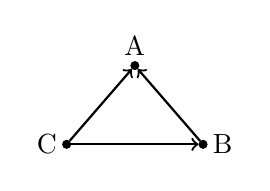
\begin{tikzpicture}

\def\point{node [circle, draw, fill, inner sep = 0, minimum size = .1cm] }

\draw (0, 1cm) \point (A) {};
\draw (0.866cm, 0) \point (B) {};
\draw (-0.866cm, 0) \point (C) {};

\node [above] at (A) {A};
\node [right] at (B) {B};
\node [left] at (C) {C};

\draw[->, thick] (C) -- (A);
\draw[->, thick] (C) -- (B);
\draw[->, thick] (B) -- (A);

\end{tikzpicture}
\caption{Результат голосования.}
\end{figure}

Я упорядочил этот список по убыванию количества отданных голосов. Если бы в этом списке оказалось два одинаковых значения (например, $X>Y$ и $T>U$), то мы сравнили противоположные пары ($Y>X$ и $U>T$) и поставили бы выше ту, которая имеет меньше голосов за противоположный вариант. Теперь, используя этот упорядоченный список, мы начинаем рисовать ориентированный граф, вершинами которого являются кандидаты. Мы начинаем рисовать рёбра последовательно от начала списка к концу, проская те рёбра, в результате которых образуется цикл. На рисунке~3.17 показан результирующий граф для нешего примера. На таком графе окажутся вершины, из которых исходят рёбра, но в которые рёбра не заходят. Такая вершина показывает победителя выборов (в нашем случае $C$). Докажите, что, такая система голосования всегда выберет победиля по Кондорсе, если таковой имеется, что она никогда не выберет проигравшего по Кондорсе, и что введение фиктивных кандидатов (походих на существующих кандидатов, если они не фавориты) не повлияет на исход голосования. В некоторых случаях эта система не сможет определить победителя, что это за случаи такие?
\end{exercise}

Парадокс Кондорсе показывает, что <<честных выборов>> существовать не может по крайней мене таком смысле: предпочтения социума не транзитивны, а следовательно во многих случаях <<объективного>> победителя может и не быть. Однако, это не значит что все выборы заведомо <<нечестные>>. Во-первых, во многих случаях победитель по Кондорсе всё же существует. Во-вторых, помимо критерия победиля по Кондорсе могут быть и другие критерии: например, суммарная полезность победителя для общества, если избиратели её оценивают в ходе голосования. В конце этого параграфа мы продемонстрируем ещё несколько теорем о <<невозможности справедливых выборов>>, которые исходят уже из других предположений, но прежде покажем довольно простой результат, называемой \term{теоремой Мэя}.

\begin{thm}
Голосование простым большинством является единственной возможной системой голосования, удовлетворящей одновременно следующим критериям:
\begin{enumerate}
\item выбор осуществляется между двумя кандидатами, в результате чего либо один из них побеждает, либо объявляется ничья; каждый избиратель может голосовать либо за одного из кандидатов, либо воздержаться;
\item голования анонимны
\item сама система голосований не зависит от личности кандидатов
\item пусть в результате выборов либо объявляется ничья, либо побеждает кандидат $X$, тогда при тех же самых условиях, если один из избирателей отменит свой голос за кандидата $Y$, либо же воздержавшийся избиратель решит отдать свой голос за $X$, победит $X$.
\end{enumerate}
\end{thm}
\begin{proof}
Условия 2 и 3 означают, что если все избиратели вдруг резко сменят свой голос на противоположный, то рузультат голосований так же сменится на противоположный. Из этого следует, что если за $X$ и $Y$ проголосовало одинаковое количество человек, то результатом обязательно будет ничья: в противном случае эти условия нарушались бы.

Теперь, пусть за $X$ отдаётся на один голос больше, чем за $Y$. Это всё равно, что из состояния ничьей кто-то однал свой голос за $X$. По условию монотонности $X$ побеждает. Продолжая по индукции мы получаем, что побеждает всегда тот кандидат, за которого отдано большинство голосов.
\end{proof}

Что произойдёт в случае, если кандидатов больше, чем два? Мы уже видели, что в этом случае голосование простым большинством имеет определённые проблемы, хотя и не связанные с условиями, обозначенными в тереме Мэя. Мы докажем, что при опредлённых условиях, накладываемых на <<справедливость>>, адекватной системы голосования может и не быть вовсе.

\begin{definition}
\term{Решающим множеством} избирателей называется такая группа избирателей, что если все избиратели из этой группы проголосуют одинаково, то это результат голосования определится предпочтением этой группы. Если решающее множество избирателей состояит из одного человека, то такой избиратель называется \term{диктатором}.
\end{definition}

\begin{definition}
\term{Фильтром над множеством $X$} называется такое семейство подмножеств $\mathcal{F}\subset 2^X$, для которого выполняются следующие условия:
\begin{enumerate}
\item $\varnothing \not\in \mathcal{F}$, $X\in\mathcal{F}$;
\item если $A\in\mathcal{F}$ и $A\subset B$, то $B\in \mathcal{F}$;
\item если $A\in\mathcal{F}$ и $B\in\mathcal{F}$, то $A\cap B\in\mathcal{F}$.
\end{enumerate}
\end{definition}

Понятно, что решающее множество избирателей определено в общем случае неоднозначно, поэтому мы на самом деле можем говорить не об одном решающем множестве, а сразу о семействе множеств. Легко так же видеть, что семейство решающих множеств так же удовлетворяет всем свойствам фильтра, кроме, возможно последнего. Одной из целей нашего последующего рассуждения будет как раз показать, что последнее свойство при определённых условиях так же работает.

Интуииция про фильтры как раз может быть такой, то фильтр определяет семейство <<больших>> множеств, но не в смысле количества элементов в нём, а в смысле их значительности. Образно представить себе решето, в которое вы бросам множества, и маленькие множества проскакаивают, а большие остаются. Решето очень похоже технически на фильтр, который что-то пропускает, а что-то оставляет, отсюда и терминология.

На будущее замечу, что в определении фильра мы на самом деле никак не использовали свойства множеств, мы лишь использовали символы $\cap$ и $\subset$. Это позволяет нам ввести понятие фильра не только для булеана множеств, но и для произвольной ограниченной решётки, заменив $\subset$ на $<$ и $\cap$ на $\land$. Пока нам это не нужно, но в дальнейшем это окажется полезным.

Как и любое семейство множеств, все фильтры на $X$ можно упорядочить используя отношение включения. В этом смысле следует понимать следующее определение.

\begin{definition}
\term{Ультрафильтром} называется максимальный фильтр.
\end{definition}

\begin{example}
Рассмотрим семейство всех подмножеств $X$, содержащих в качестве элемента некоторый фиксированный $x$. Обозначим это семейство за $<x>$. Легко проверить, что это фильтр, однако $<x>$ так же является и ультрафильтром. Если предположить, что $<x>$ не ультрафильтр, то должен существовать какой-то более <<крупный>> фильтр $\mathcal{F}$, содержащий в себе $<x>$, но он в свою очередь должен содержать в себе множество без элемента $x$. Такое множество будет иметь пустое пересечение с $\{x\}\in<x>$ что нарушает свойство 3 фильтра. Про ультрафильтры $<x>$, что они \term{порождены} элементом $x$
\end{example}

Мы покажем ниже, что, во-первых решающее множество является не просто фильтром, но ультрафильтром, а так же что любой ультрафильтр над конечным множеством порождён единственным элементом. Следовательно, существует диктатор.

\begin{definition}
Мы будем говорить, что семейство множеств обладает свойством \term{FIP}, если любое конечное пересечение элементов этого множества непусто (FIP расшифровывается как Finite-Intersection property, что дословно и переводится как <<свойство конечного пересечения>>).
\end{definition}

\begin{lemma}
Любое FIP-семейство подмножеств $X$ может быть расширено (путём добавления в него новых множеств) до ультрафильра.
\end{lemma}
\begin{proof}
Во-первых, добавим в семейтсво все возможные пересечения его множеств. Затем добавим для каждого множества все его надмножества (то есть для каждого $A\subset X$ добавим все множества $B\subset X$ такие что $A\subset B$). Таким образом мы получили фильтр. Обозначим его как $\mathcal{F}$.

Рассмотрим множество всех фильтров над $X$ и рассмотрим в нём максимальное линейно-упорядоченное подмножество $F_0\subset F_1\subset F_2, \ldots$ (такие подмножества называются \term{цепью}), содержащее в качетсве элемента $\mathcal{F}$. Поскольку все элементы цепи являются подмножествами конечного множества, сама цепь будет конечна, и таким образом в ней найдётся максимальный элемент, который и будет расширением $\mathcal{F}$ до ультрафильтра.

В случае бесконечных множеств доказательство будет очень похожим, но потребует несколько более экстравагантного математического аппарата, который мы введём в пятой граве (доказательство останется тем же, только мы добавим фразу <<по лемме Цорна существует максимальный элемент>>). Пока бесконечный случай нам не потребуется.
\end{proof}

\begin{lemma}
Пусть $\mathcal{F}$~--- ультрафильтр, и $B$ такое множество, что $\forall A\in\mathcal{F}$ пересечение $A\cap B$ непусто. Тогда $B\in\mathcal{F}$.
\end{lemma}
\begin{proof}
Легко увидеть, что семейство множеств $\mathcal{T} = \{B\cap A| A\in\mathcal{F}\}$ обладает свойством FIP, а следовательно может быть расширено до некоторого ультрафильтра $\mathcal{G}$. Однако ультрафильтр $\mathcal{F}$ сам является расширением до ультрафильтра семейства $\mathcal{T}$, и в силу максимальности, отсюда следует, что $\mathcal{G} = \mathcal{F}$. Однако мы знаем, что $B\in\mathcal{T}$, откуда следует утверждение леммы.
\end{proof}

\begin{lemma}
Если $A\cup B\in\mathcal{F}$ и $\mathcal{F}$~--- ультрафильтр, то по крайней мере одно из множеств $A$ или $B$ ему принадлежит.
\end{lemma}
\begin{proof}
Прежположим, что $A,B\not\in\mathcal{F}$. Возьмём такие $C, D\in\mathcal{F}$, что $A\cap C = B\cap D = \varnothing$. Такие множества мы всегда можем выбрать, так как если бы это не удалось, то по прошлой лемме $A$ или $B$ принадлежали бы ультрафильтру. Но при таком выборе $(A\cup B)\cap(C\cap D) = \varnothing$, и, поскольку $C\cap D\in\mathcal{F}$, по третьему свойству фильтров, $A\cup B \not\in \mathcal{F}$. Полученное противоречие завершает доказатальство леммы.
\end{proof}

\begin{thm}
Для того, чтобы фильтр $\mathcal{F}$ над $X$ был ультрафильтром, необходимо и достаточно, чтобы для любого множества $A$ выполнялось либо $A\in\mathcal{F}$, либо $A^C\in\mathcal{F}$.
\end{thm}
\begin{proof}
Пусть $\mathcal{F}$ ультрафильтр. Мы знаем, что $A\cup A^C = X \in\mathcal{F}$. Утверждение теоремы следует из последней леммы.


В обратную сторону. Если указанное свойство выполняется, то это значит, что мы никак не можем расширить фильтр. Рассмотрим, например, мы множество $B$, такое что $A\subset B\not\in\mathcal{F}$. Но тогда $B^C\in\mathcal{F}$, хотя $A\cap B^C=\varnothing$, что противоречит свойству фильтра.
\end{proof}

\begin{corollary}
Любой ультрафильтр над конечным множеством имеет вид $<x>$.
\end{corollary}
\begin{proof}
Если $A$ и $B$ непересакаются и их объединение принадлежит ультрафильтру, то ровно одно из этих множеств принадлежит фильтру. Рассуждая по индукии можем получить, что если
$$\cup_{i=1}^n A_i = X$$
для непересекающихся $A_i$, то ровно одно из них принадлежит ультрафильтру. Теперь, если $X$~--- конечное множество, то в качестве $A_i$ можно взять одноэлементные множества. Доказываемое следует отсюда немедленно.
\end{proof}

В пятой главе мы покажем, что на бесконечных множествах бывают и другие ультрафильтры (любой элемент в ультрафильтре тогда будет бесконечным множеством), для текущих же целей нам достаточно знать лишь о конечных множествах. Из данного следствия сразу видно, что если мы докажем, что семейство решающих множеств~--- это ультрафильтр, то найдётся и одноэлементное решающее множество, то есть диктатор. Теперь мы готовы доказать нашу основную теорему.

\begin{thm}
(Гибберт-Саттервайте) Любая система выборов, в которой может победить любой из кандидатов (при соответствующих голосах за него), и в которой невозможно тактическое голосование, будет иметь диктатора.
\end{thm}

Прежде чем перейти к непосредственному доказательству, уточним немного формулировку и получим парочку лемм. Множество кандидатов будем обозначать как $[m]$, множество избирателей как $[n]$. Избиратель $i\in [n]$ имеет предпочтения, выражающиеся перестановкой, которые мы будем обозначать как $\pi_i$. Тогда место, на которое поставил бы избиратель кандидата $x$ обозначается как $\pi_i(x)$. Сама функция голосования~--- это функция типа $f:S_m^n\to [m]$. Элемент множества $S_m^n$ будем называть \term{профилем голосования}. Для краткости будем обозначать $P = S_m^n$. Соответственно конкретное голосование~--- это элемент $\pi\in P$.

Определим строго что значит <<невозможно тактическое голосование>>. Тактической голосование~--- это когда некий избиратель $i$ записывает в биллютень не реальные свои предпочтения, а некоторые другие. В итоге профиль $\pi$ меняется на $\pi'$. Если при этом $\pi_i(f(\pi')) > \pi_i(f(\pi))$, то это значит, что избиратель $i$ смог как-то сманипулировать выборами в свою пользу. Это и значит, что произошло тактическое голосование. Условия теоремы предполагают, что это должно быть невозможно.

\begin{lemma}
Пусть $\pi, \pi'\in P$ и $f(\pi) = a$ и пусть
$$\forall i\in [n]\ \forall x\in[m]\ \pi_i(a)\ge\pi_i(x)\to\pi'_i(a)\ge\pi'_i(x)$$
Тогда $f(\pi') = a$.
\end{lemma}

Это значит, что если какие-то кандидаты поменяют свои предпочтения на новые, не изменив свои предпочтения относительно $a$ в негативную сторону, то и результат голосования так же не поменяется.

\begin{proof}
Пусть вначале для определённости свой голос меняет лишь один избиратель с номером 1 (обозначим его новые предпочления как $\pi_1'$). Предположим, что $f(\pi') = b$. По условию невозможности манипуляций, это значит, что $\pi_1(b)\le\pi_1(a)$ и, по предположению леммы, $\pi_1'(b)\le\pi_1'(a)$. Если теперь рассмотреть профиль $\pi'$ и вернуть предпочтения избирателя 1 в первоначальное состояние, то по тому же принципу выяснится, что $\pi_1'(b)\ge\pi_1'(a)$. Это значит, что $a=b$. Осталось последовательно провести применить процедуру для всех избирателей и мы получаем утверждение леммы.
\end{proof}

\begin{lemma}
В условиях теоремы Гибберта-Саттервайте, если все избиратели больше предпочитают $a$, нежели $b$, то $b$ не может победить.
\end{lemma}
\begin{proof}
Пойдём от противного. Пусть $\pi$ ~--- такой профиль голосвания, что все избиратели предпочитают $a$ над $b$, но в то же время $f(\pi) = b$. Поскольку по условиям каждый кандидат может победить, существует так же профиль голосования $\pi'$ такой что $f(\pi') = a$. Рассмотрим так же профиль голосования $p$ такой, что он соответствует целиком профилю $\pi$ за исключением того, что $a$ и $b$ у него находятся в самом верху предпочтений (причём по условию $a$ предпочтительнее $b$). По прошлой лемме $b = f(\pi) = f(p)$, поскольку $p$ получается из $\pi$ путём лишь повышения предпочительности $b$ у всех кандидатов. В то же время $a = f(\pi') = f(p)$, поскольку $p$ можно получить и из $\pi'$ тем же способом, единственное отличие тут в том, что в некоторых случаях $a$ переместится выше $b$, что опять же не должно влиять на победу $a$ по прошлой лемме. Получаем, что $a=b$. Полученное противоречие завершает доказательство леммы.
\end{proof}

Фиксируем некоторых кандидатов $x$ и $y$. Пусть $S$~--- такое множество избирателей, что если все они предпочитают $x$ над $y$, то $y$ не может победить. Множество $S$, вероятно, неединственное такое, и семейство всех таких множеств мы обозначим как $\mathcal{F}_{xy}$. Нам предстоит доказать две вещи. Во-первых, что $\mathcal{F}_{xy}$ не зависит от $x$ и $y$. Это значит, что для любой пары кандидатов такие семейства совпадают, поэтому такие семейства являются как раз решающим множеством. И, во-вторых, мы докажежем, что это семейство является ультрафильтром.

Обозначим за $V_{xy}(\pi)$ всех избирателей, которые предпочитают $x$ над $y$ в профиле голосования $\pi$ и перечислим несколько простых свойств семейства $\mathcal{F}_{xy}$:

\begin{enumerate}
\item $\mathcal{F}_{xy}$ непусто, так как по крайней мере $[n]\in\mathcal{F}_{xy}$;
\item Пусть $S\subset T$ и $S \in \mathcal{F}_{xy}$, тогда $F\in\mathcal{F}_{xy}$
\item $S\in\mathcal{F}_{xy} \leftrightarrow S^C\not\in\mathcal{F}_{yx}$
\end{enumerate}

Эти свойства довольно очевидны, они соостветствуют первым двум свойствам фильтров а так же теореме 3.50. Если доказать, что $S\cap T\in\mathcal{F}_{xy}$ для любых множеств $S, T\in\mathcal{F}_{xy}$, то это завершит доказательство, что $F_{xy}$ ультрафильтр. Нам понадобится следующая

\begin{lemma}
$S\in\mathcal{F}_{xy} \leftrightarrow \exists \pi\ V_{xy}(\pi) = S \land f(\pi) = x$
\end{lemma}
\begin{proof}
Чтобы увидеть следствие слева направо, достаточно взять профиль голосования, при которой все избиратели ставят $a$ и $b$ наиболее предпочтительными над остальными, но только избиратели из $S$ предпочитают $a$.

Докажем это в обратную сторону от противного. Пусть $\pi$ и $\pi'$~--- такие профили, что $x>y$ в точности для избирателей из $S$, причём $f(\pi)=x$ (такой существует по предположению леммы) и $f(\pi') = y$. Если изменить эти профили таким образом, что $x$ и $y$ будут на самом верху предпочтений для всех избирателей, то результаты голосования не изменятся по лемме 5: в обоих случаях победить могут либо $x$ либо $y$, т.к. их предпочитают все избиратели. После такого пробразования изменение предпочтений между прочими кандидатами не имеет значения для исхода голосования опять же по лемме 5. Это, однако, проводит к противоречию, так как и в $\pi$ и $\pi'$ относительный порядок $x$ и $y$ одинаков для одних и тех же избирателей: изменением кандидатов, отличных от $x$ и $y$ получается что можно поменять победителя, что невозможно.
\end{proof}

\begin{lemma}
$\forall x, y, z, t\ \mathcal{F}_{xy} = \mathcal{F}_{zt}$
\end{lemma}
\begin{proof}
Докажем вначале, что $\mathcal{F}_{xy}\subset\mathcal{F}_{yz}$. Рассмотрим профиль голосования $\pi$ и множества $S\in \mathcal{F}_{xy}$ и $T\in\mathcal{F}_{yz}$ такие, что:
\begin{enumerate}
\item $x > z > y$ для избирателей из $S\backslash T$;
\item $x>y>z$ для избирателей из $S\cap T$;
\item $y>z>x$ для избирателей из $T\backslash S$;
\item $z>y>z$ для избирателей из $(S\cup T)^C$;
причём кандидаты $x, y, z$ предпочтительнее любого другого кандидата для любого избирателя. По лемме 5 в таком голосовани победить может только один из них троих. Однако $y$ победить не может, так как $S\in\mathcal{F}_{xy}$, и все избиратели из $S$ предпочитают $x>y$. По тем же соображениям не может победить и $z$, поскольку для всех избирателей из множества $T\in\mathcal{F}_{yz}$, $y$ предпочтительнее. Имеем в итоге, что $f(\pi)=x$ и по лемме~6 получается, что $S\in\mathcal{F}_{xz}$. Это доказывает, что $\mathcal{F}_{xy}\subset\mathcal{F}_{xz}$.

Совершенно аналогично можно показать, что так же и $\mathcal{F}_{xz}\subset\mathcal{F}_{xy}$, то есть что $\mathcal{F}_{xy}=\mathcal{F}_{xz}$. Аналогичным образом можно так же показать, что и $\mathcal{F}_{xy}=\mathcal{F}_{xy}$. Таким образом все семейства $F_{xy}$ не зависят от выбора $x$ и $y$ и являются определяющими множествами.
\end{enumerate}
\end{proof}

